\hyphenation{wnio-sko-wa-nie}
\chapter{Problematyka automatycznego planowania}
\section{Opis dziedziny}
Automatyczne planowanie to poddziedzina sztucznej inteligencji. Dotyczy wykonywania sekwencji akcji, realizacjii strategii lub generowania planów, prowadzących do określonego wyniku.

Każdy problem automatycznego planowania zawiera stan początkowy oraz stan końcowy. W stanie początkowym określone są wszystkie wartości zmiennych (stany poszczególnych obiektów) jakie aktualnie zawarte są w problemie, a które mają zostać zmienione podczas wykonania planu. W stanie końcowym sformułowane są wartości zmiennych, kórych osiągniecie jest głównym zadaniem planu. Ponad to problemy automatycznego planowania zawierają zdefiniowane akcje, umorzliwiające zmianę stanów. Tylko przez podejmowanie akcji plan może zostać wykonany. Wyjątkiem jest sytuacja, w której stan końcowy jest równy stanu początkowemu.

Plany, otrzymywane w wyniku rozwiązywania problemów, można otrzymać dzięki zastosowaniem różnego rodzaju schematów działania. Spośród klasycznych algorytmów, wymienić można między innymi całkowity przegląd stanów, wnioskowanie w tył czy wnioskowanie w przód. Mimo, iż całkowity przegląd stanów zapewni rozwiązanie najlepsze, jest to rzadko stosowane rozwiązanie. Liczba stanów możliwych do osiągnięcia rośnie wykładniczo, co powoduje, że zaplanowanie nawet niezbyt skomplikowanych problemów, może zająć czas, w którym rozwiązanie znacznie przekracza zdatność do użycia. W takim wypadku stosuje się algorytmy mogące zwrócić plany, których wykonanie zajmie więcej czasu, jednak szybkość ich uzyskania znacznie wzrasta.

Pomimo zwracania satysfakcjonujących wyników przez algorytmy klasyczne, wykorzystywane jest również kilka bardziej złożonych rozwiązań.Jednym z nich jest przekształcenie danego problemu automatycznego planowania w inny,a następnie  rozwiązanie go najlepszą znaną metodą. Kolejnym wyjściem są algorytmy probabilistyczne. Polegają one na polepszaniu wyników podczas kolejnych iteracji. Algorytmy te wykonują akcje z określonym prawdopodobieństwem, przez co, może się okazać, że optymalny plan zostanie uzyskany później niż w przypadku pełnego przeglądu stanów, lub nawet nie zostanie uzyskany nigdy. Na ogół jednak, algorytmy probabilistyczne dosarczają wyniki porównywalne z algorytmami klasycznymi, w nie gorszym czasie.

Bardzo często, w celu zademonstrowania czym jest automatyczne planowanie, stosuje się układ złożony z klocków, umiejscowionych w określonej pozycji. Zadaniem algorytmów planowania jest takie ułożenie akcji, aby stan końcowy położenia klocków zgadzał się ze stanem aktualnym. 

Przykładowo, istnieją 3 klocki, nazwane odpowiednio x,y,z. Każdy z nich może być podniesiony lub umiejscowionym na jednym z dwóch dostępnych pól, czy na innym klocku, pod warunkiem, że ten nie jest akurat podniesiony i nic się na nim nie znajduje. Dla danego problemu zdefiniowane zostały akcje podnieś, która podnosi dany klocek, oraz połóż, dzieki której można umiejscowić obiekt na wolnym miejscu lub obiekcie.Stan początkowy zdefiniowany jest następująco: klocek z położony jest na pierwszym miejscu,klocek y położony jest na klocku z, a klocek x na klocku y. Stan końcowy wygląda tak, że klocek x znajduje się na miejscu drugim, na nim umiejscowiony jest klocek y, a z kolei na nim klocek z. Inaczej można przedstawić to w języku predykatów:
\\\\
Stan początkowy:
\\\\
\textit{P=\{wolny(x),na(x,y),na(y,z),na(z,M1)\}}
\\\\
Stan końcowy:
\\\\
\textit{K=\{wolny(z),na(z,y),na(y,x),na(x,M2)\}}

Na rysunku (rys.~\ref{fig:automatyczne-planowanie}) przedstawiono graficzne odwzorowanie stanu początkowego i końcowego.
\begin{figure}[h!]
    \centering
    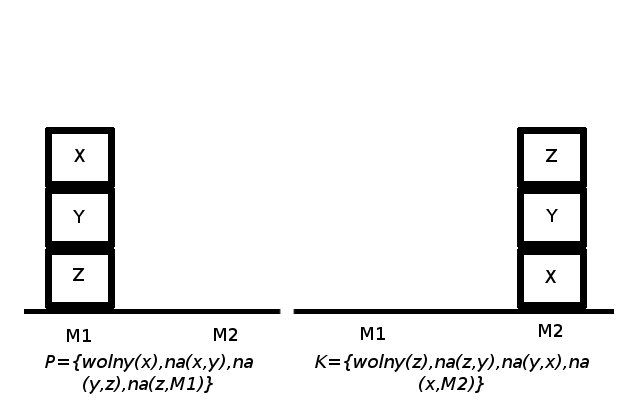
\includegraphics[width=0.5\textwidth]{img/rys2,1}
    \caption{Graficzna reprezentacja stanu początkowego i końcowego}
    \label{fig:automatyczne-planowanie}
\end{figure}


\section{Język PDDL}
W celu polepszenia wydajności automatycznego planowania, stworzone zostało kilka formalnych języków. Najpopularniejsze z nich to STRIPS (\textbf{St}anford \textbf{R}esearch \textbf{I}nstitute \textbf{P}roblem \textbf{S}olver), ADL (Action description language) oraz PDDL (Planning Domain Definition Language). PDDL, który stworzony został najpóźniej, jest wzorowany na dwóch pozostałych językach. Został utworzony przez Drew McDermott'a w roku 1998. Celem jego stworzenia był Międzynarodowy konkurs planistyczny (International Planning Competition),który bez odpowieniego narzędzia nie mógłby się odbyć.

Od pojawienia się pierwszej wersji języka w roku 1998, jest on systematycznie rozwijany. Kolejne wersje 2.1, 2.2, 3.0, oraz najnowsza 3.1 zostały użyte na międzynarodowych konkursach w latach 2002, 2004, 2006, 2008. Oprócz standardowych wersji języka, rozwijane są inne, niezależne warianty. Pośród nich znajdują się między innymi PDDL+, w którym zawarto procesy i zdarzenia, Web-PDDL umożliwiający wyrażenie przestrzeni nazw za pomocą URI (Uniform Resource Identifier), czy NDDL (New Domain Definition Language), różniący się używaniem zmiennych oraz interwałów zamiast akcji.

Problemy automatycznego planowania, przedstawione w języku PDDL, są zapisane w dwóch plikach, domeny oraz problemu. Poniżej przedstawiono skrócony opis obydwu plików. Składa się on z przedstawienia elementu, krótkiego opisu oraz przykładu.
\\\\\\
Plik domeny zawiera:
  \begin{itemize}
\item Domena - definicja domeny - \textit{(define (domain samoloty))}
\item Rozszerzenie - domena zawierająca dany wpis dziedziczy wymagania, typy, stałe, akcje, aksjomaty z innej domeny - \textit{(:extends pojazdy) }
\item Wymagania - wymagania oczekiwane przez domenę - \textit{(:requirements :strips :typing)}
\item Typy - typy znajdujące się w domenie - \textit{(:types okno drzwi)}
\item Stałe - zdefiniowane stałe - \textit{(:constants pierwsza druga - opona)}
\item Zmienne domeny - zmienne dla domen, które mają zadeklarowe wymaganie :expression-evaluation - \textit{(:domain-variables zmienna - int)}
\item Predykaty - lista predykatów zawartych w domenie (znak ? poprzedzający x oznacza, że x jest zmienną) -  \textit{(:predicates (na-lotnisku ?x))}
\item Pola wieczne - lista literałów, które są prawdziwe w każdej chwili - \textit{(:timeless literał (nazwa))}
\item Ograniczenia bezpieczeństwa - cele drugoplanowe, które muszą zostać spełnione - \textit{(:safety (:goal (na-lotnisku samolot))}
\item Akcje - akcje, których podejmowanie ma zapewnić osiągnięcie celu - \textit{(:action laduj :parameters (?s - samolot ?l - lotnisko ?p - powietrze) :precondition (jest-na ?s ?p) :effect (jest-na ?s ?l)) }
\end{itemize}

Poniżej zaprezentowano zawartość przykładowego pliku domeny:\\\\
\textit{(define (domain loty)\\
(:extends pojazdy)\\
(:requirements :strips :typing )\\
(:predicates\\	
\hspace*{1cm}(lotnisko ?m - miejsce)\\
\hspace*{1cm}(powietrze ?m - miejsce)\\
\hspace*{1cm}(samolot	?p - pojazd)\\
{  } (jest-na ?p - pojazd ?m - miejsce)\\ 
)\\
  (:action laduj\\
   :parameters (?s - samolot ?m - miejsce)\\ 
\hspace*{1cm}:precondition (is-at ?s ?m) \\
\hspace*{1cm}:effect (jest-na ?s ?m) \\
)\\
)} \\

Plik problemu zawiera:
\begin{itemize}
\item Domena - opis zawarty w poprzednim akapicie - \textit{(:domain loty)}
\item Wymagania - opis zawarty w poprzednim akapicie
\item Sytuacja - nazwa sytuacji początkowej - \textit{(:situation początek)}
\item Obiekty - lista obiektów problemu - \textit{(:objects drzewo liść)}
\item Stan początkowy - stan początkowy problemu - \textit{(:init (jest A) (w B hangar))}
\item Cel - oczekiwany stan końcowy problemu - \textit{(:goal (and (jest A) (w C hangar) (w B lotnisko))}
\item Długość rozwiązania - pole stwierdzające, iż istnieje rozwiązanie o podanej długości - \textit{(:length (:serial 5))}
\end{itemize}

Poniżej zaprezentowano zawartość przykładowego pliku problemu:\\\\
\textit{(define (problem lotniska-start)\\
\hspace*{1cm}(:domain lotniska)\\
\hspace*{1cm}(:situation lądowanie)\\
\hspace*{1cm}(:init (at B hangar) (at A lotnisko))\\
\hspace*{1cm}(:goal (and(at A hangar) (at B lotnisko))))}


\section{Oprogramowanie}
Aby język PDDL mógł spełniać swoją rolę, wymagane są narzędzia służące do planowania. Jednym z takich przyrządów jest \textit{Fast Downward}. Pozwala na zaplanowanie problemu zapisanego w jęzeku PDDL w wersji 2.2. Dodatkowo wspiera wymaganie \textit{:action-costs}, używane w wersji 3.1. Aplikacja wymaga od użytkownika posiadania wiersza poleceń oraz prostego edytora tekstu. Du ułożenia planu \textit{Fast Downward} używa heurestyki opartej na algorytmie \textit{Best-First Search}. Na podobnej zasadzie działania oparte są aplikacje \textit{Fast Forward} oraz \textit{LPG}.

Kolejny elektroniczny planista nosi nazwę \textit{Satplan}. Algorytm wykorzystywany przez ten program spełnia założenia metody automatycznego planowania o takiej samej nazwie: konwertuje daną instancje problemu planowania na instancje problemu spełnialności, a następnie rozwiązuje wykorzystując odpowiednie schematy działań. Algorytm zawarty w \textit{Satplanie} ma następujący przebieg: utworzenie grafu planistycznego do pewnej długości \textit{k}, zamiana więzi wynikających z grafu na zbiór klauzul, używając odpowiedniego algorytmu pozwalającego rozstrzygnąć problem spełnialności, znajduje się odpowiednie rozwiązanie. W przypadku gdy nie można było znaleźć wyniku, zwiększona zostaje wartość \textit{k}. Jeśli jednak rozwiązanie zostało znalezione, transponuje się wynik działania algorytmu do wyniku pierwotnego pierwotnego problemu planowania. Na końcu usuwane są niektóre z niepotrzebnych akcji.

Kolejną aplikacją umożliwiającą rozwiązywanie problemów automatycznego planowania jest \textit{Gavs+ (Game Arena Visualization and Synthesis, Plus!)}, który skupia się na kwestiach związanych z grami. Program ten posiada bibliotekę (\textit{PDDL4J}) umożliwiającą wykonywanie problemów zapisanych w PDDL. Dzięki wbudowanemu interfejsowi \textit{Gavs+} umożliwia graficzne prześledzenie wynikowego planu.

Wszystkie opisane tu narzędzia stworzone zostały na licencji otwartego oprogramowania.

%algorytmy używane przez planery
%satplan
%gavs +
